\chapter{Inférence pour la RLM}
\label{sec:InferenceRLM}


\section{Distribution de l'estimateur}

Comme dans le cas de la RLS, on utilisera la distribution des estimateurs pour dériver les méthodes d'inférence.  Pour trouver la loi des estimateurs, on doit faire l'hypothèse que la matrice des termes d'erreurs $\boeps$ est distribuée selon une loi normale multivariée de dimension égale au nombre d'observations $n$. Une brève introduction à cette distribution multivariée est présentée à l'annexe \ref{LaLoiNormaleMultivariée}.

On peut écrire cette hypothèse sous la forme
$$\boeps=[\varepsilon_1,\varepsilon_2,...,\varepsilon_n]' \sim \N_n(\textbf{0}, \sigma^2\boI_n)$$
où  $\boI_n$ dénote la matrice identité de dimension $n\times n$.

On a donc que
\begin{eqnarray*}
	\boY \sim \N_n (\boX\bobeta, \sigma^2 \boI_n).
\end{eqnarray*}

Afin de déterminer l'espérance et la variance de $\hbobeta$ on suit la même approche que pour la régression linéaire simple et on exprime $\hbobeta$ comme une combinaison linéaire des $Y_i$.


On a vu que
\begin{eqnarray*}
	\hbobeta=(\boX'\boX)^{-1}\boX'\boY
\end{eqnarray*}
On a donc que $\hbobeta \sim \N_p(\esp[\hbobeta],\var[\hbobeta])$ car une combinaison linéaire de variables aléatoires normales est également normalement distribuée. Il suffit donc de calculer $\esp[\hbobeta]$ et $\var[\hbobeta]$ afin que la distribution soit entièrement déterminée.

On peut d'abord montrer que l'estimateur est non biaisé:
\begin{eqnarray*}
	\esp[\hbobeta]&=&\esp[(\boX'\boX)^{-1}\boX'\boY] \\
	&=& (\boX'\boX)^{-1}\boX' \esp[\boY]\\
	&=& (\boX'\boX)^{-1}\boX' \boX\bobeta\\
	&=& \bobeta
\end{eqnarray*}
On calcule ensuite la variance:
\begin{eqnarray*}
	\var[\hbobeta]&=& \var[(\boX'\boX)^{-1}\boX'\boY]\\
	&=& (\boX'\boX)^{-1}\boX' \var[\boY] \left\{(\boX'\boX)^{-1}\boX'\right\}'\\
	&=& (\boX'\boX)^{-1}\boX' \sigma^2\boI_n \left\{(\boX'\boX)^{-1}\boX'\right\}'\\
	&=& \sigma^2 (\boX'\boX)^{-1} \boX' \boX(\boX'\boX)^{-1}\\
	&=& \sigma^2 (\boX'\boX)^{-1}
\end{eqnarray*}
Donc,
\begin{eqnarray}
	\hbobeta \sim \N_p\{\bobeta,\sigma^2 (\boX'\boX)^{-1}\}
	\label{loibeta}
\end{eqnarray}


\subsubsection{Application au cas $p=1$}
\label{sec:VarCovDesEstimateur}

On a déjà vu que dans le cas où $p=1$,

\begin{equation}
\label{invxtx}
\begin{MAT}{c}
(\boX' \boX) ^{-1}\\
\end{MAT}
 =
\begin{MAT}{c}
\frac{1}{nS_{xx}}\\
\end{MAT}
\left[
\begin{MAT}(e){cc}
\sum_{i=1}^n x_i^2 & -n\bar{x}\\
-n\bar{x} & n \\
\end{MAT}
\right].
\end{equation}

À partir de \eqref{loibeta} et \eqref{invxtx}, on peut calculer les variances et la covariance de $\hat{\beta}_0$ et de $\hat{\beta}_1$.

\begin{eqnarray*}
	\var[\hat{\beta}_1]&=&\frac{\sigma^2 n}{n S_{xx}} = \frac{\sigma^2}{S_{xx}}\\
	\var[\hat{\beta}_0]&=&\frac{\sigma^2 \sum_{i=1}^n x_i^2}{n S_{xx}}\\
	\cov[\hat{\beta}_1,\hat{\beta}_0]&=& \frac{-n\bar{x} \sigma^2}{n S_{xx}}= \frac{-\bar{x} \sigma^2}{S_{xx}}
\end{eqnarray*}

On obtient les variances déjà connues. Remarquez que la covariance entre $\hat{\beta}_0$ et $\hat{\beta}_1$ est de signe contraire de $\bar{x}$ et que cette covariance est nulle si $\bar{x}=0$. %Dans le cas où $p=2$, on trouve
%%
%
%\begin{eqnarray*}
%		f(X_1,X_2)= \left(\frac{1}{\sqrt{2\pi}}\right)^2 \frac{1}{\left|\Sigma\right|^{1/2}} \exp\left(-\frac{1}{2} (X- \mu)^T \Sigma^{-1} (X- \mu)\right)\\
%		= \left(\frac{1}{\sqrt{2\pi}}\right)^2 \frac{1}{\sigma_1\sigma_2\sqrt{1-r^2}} e^{ -\frac{1}{2 (1-r^2)} \left(\frac{x_1- \mu_1}{\sigma_1}\right)^2 +\left(\frac{x_2- \mu_2}{\sigma_2}\right)^2 - 2r\left(\frac{x_1- \mu_1}{\sigma_1}\right)\left(\frac{x_2- \mu_2}{\sigma_2}\right)}
%\end{eqnarray*}
%
%Le dernier terme de l'exponentielle est un terme croisé qui induit la corrélation; il est nul lorsque $r$, la corrélation entre $X_1$ et $X_2$ est égale à zéro.



\section{Matrice chapeau et implications}
\label{sec:MatriceChapeau}

On a introduit la matrice chapeau à la section \ref{sec:ArgumentGéométrique}. Cette matrice est très importante dans la RLM. Dans cette section, on explore plus en détails la matrice chapeau, et on obtient quelques résultats utiles pour l'inférence à partir de ses propriétés.

\subsection{La matrice chapeau}
\label{sec:LaMatriceChapeau}

La matrice chapeau $\boH$ («hat matrix») tire son nom du fait qu'elle permet de transformer $\boY$ en $\hY$ ("Y chapeau"). On va déterminer cette matrice. Selon l'équation \eqref{eq:reg_lin_mult_mat}, la régression linéaire multiple s'exprime sous format matriciel comme $\boY = \boX\bobeta + \boeps$.
L'estimateur de $\bobeta$ peut s'écrire selon l'équation \eqref{eq:est_beta} comme $\hbobeta = (\boX'\boX)^{-1}\boX'\boY$. On obtient donc que
\begin{eqnarray*}
	\hY& =& \boX\hbobeta \\
    &= & \boX(\boX'\boX)^{-1}\boX'\boY=\boH\boY
\end{eqnarray*}
La matrice chapeau correspond donc à la matrice $\boH=\boX(\boX'\boX)^{-1}\boX'$.


Il est également possible d'exprimer les résidus en fonction de la matrice chapeau de la manière suivante :
	\[\hboeps=\boY-\hY = (\boI_n- \boX(\boX'\boX)^{-1}\boX')\boY = (\boI_n-\boH)\boY
\]

% a continuer ici
La matrice chapeau peut être vue comme une matrice de transformation. Il s'agit d'un opérateur linéaire, de même que ($\boI_n-\boH$). Ces deux opérateurs possèdent plusieurs propriétés intéressantes, à savoir :

\begin{enumerate}
   \item $\boH'=\boH$ (symétrie)
	\item $\boH\boH=\boH$ (idempotence)
	\item $\boH\boX=\boX$
     \item $(\boI_n-\boH)'=(\boI_n-\boH)$ (symétrie)
	\item $(\boI_n-\boH)(\boI_n-\boH)=(\boI_n-\boH)$ (idempotence)
	\item $(\boI_n-\boH)\boX=0$
\end{enumerate}

De plus, tous les éléments de la matrice ont une interprétation précise et utile pour étudier la robustesse d'un modèle de RLM. Nous y reviendrons à la section \ref{sec:DonneesInfluentes}.


\subsection{Distribution de $\hat{Y}$ et $\hat{\varepsilon}$}
\label{sec:distYhatEps}

Les propriétés de la matrice chapeau permettent de calculer la variance de $\hY$ et $\hboeps$.
En effet,
\begin{eqnarray*}
	\var[\hY] = \var[\boH\boY]=\boH'\var[\boY]\boH= \boH\boH \sigma^2 = \boH \sigma^2
\end{eqnarray*}
et
\begin{eqnarray*}
	\var[\hboeps]=\var[(\boI_n-\boH)\boY]= (\boI_n-\boH)\sigma^2
\end{eqnarray*}

On a donc que les lois de $\hY$ et $\hboeps$ sont respectivement
\begin{eqnarray*}
	\hY \sim \N_n(\boX\bobeta, \sigma^2\boH)
\end{eqnarray*}
\begin{eqnarray}
	\hboeps \sim \N_n(0, \sigma^2(\boI_n-\boH)).
	\label{distepsilon}
\end{eqnarray}


\subsection{Estimation de $\sigma^2$}
\label{sec:RLM-sigma}

Comme on a indiqué à la section \ref{sec:RLM-MLE}, la méthode du maximum de vraisemblance permet de trouver un estimateur pour $\sigma^2$, mais celui-ci est biaisé. On utilisera plutôt l'estimateur suivant:
\begin{eqnarray}
	\hat{\sigma^2}=\frac{\hboeps'\hboeps}{n-p'}
	\label{estimationSigma}
\end{eqnarray}

où $p'=p+1$.

On utilisera ici le résultat \ref{distepsilon} pour prouver que \ref{estimationSigma} est non biaisé pour $\sigma^2$.


On veut donc prouver que
$$ E \left( \frac{\hboeps'\hboeps}{n-p'} \right) = \sigma^2. $$

Puisque $\hboeps \sim \N_n(0, \sigma^2(\boI_n-\boH))$, on peut écrire
$$ \frac{\hboeps}{\sigma} \sim \N_n(0, (\boI_n-\boH)).$$

On peut également écrire
$$ \frac{\hboeps}{\sigma} = (\boI_n - \boH)\bo Z \mbox{    o\`u  } \bo Z \sim \N_n(\bo 0, \boI_n).$$

\newpage
Cette forme nous permet d'utiliser le théorème suivant:

\textcolor{red}{ XXXX \\ A changer, le thm est dans le chapitre 4  maintenant. \\ XXXX}

\begin{theorem}
Si $\boY \sim \N_n(\bo 0,\boI_n)$ et $\bo A$ est une matrice symétrique, alors $\boY'\bo A\boY \sim \chi^2_r$ si et seulement si $\bo A$ est idempotente de rang r.
\end{theorem}

En effet, puisque
\begin{itemize}
\item[$\bullet$] $\bo Z \sim \N_n(\bo 0,\boI_n)$
\item[$\bullet$] $(\boI_n-\boH)$ est symétrique
\item[$\bullet$] $(\boI_n-\boH)$ est idempotente
\end{itemize}
alors, on a que
$$ \bo Z'(\boI_n-\boH) \bo Z \sim \chi^2_r$$
avec $r$ = rang$(\boI_n-\boH) = n-p'$. \\

%Si on connaît $\sigma$, il est alors possible d'utiliser ce résultat pour construire un intervalle de confiance sur $\beta_i$ ou pour faire des test d'hypothèses. Or en pratique, $\sigma$ est généralement inconnu. On l'estimera alors par

Or,
\begin{align*}
\bo Z'(\boI_n-\boH) \bo Z &= \bo Z'(\boI_n-\boH)'(\boI_n-\boH) \bo Z \\
&= ((\boI_n-\boH)\bo Z)' (\boI_n-\boH) \bo Z \\
&= \frac{\hboeps'}{\sigma} \frac{\hboeps}{\sigma} \\
&= \frac{\hboeps'\hboeps}{\sigma^2}
\end{align*}


Ainsi,
$$ \frac{\hboeps'\hboeps}{\sigma^2} \sim \chi^2_r$$
avec $r$ = rang$(\boI_n-\boH) = n-p'$. \\

On peut donc facilement prouver le résultat voulu:

\begin{align*}
E \left( \frac{\hboeps'\hboeps}{\sigma^2} \right) &= n-p' \\
E \left( \hboeps'\hboeps \right) &= \sigma^2 (n-p') \\
E \left( \frac{\hboeps'\hboeps}{n-p'} \right) &= \sigma^2
\end{align*}


\section{Intervalle de confiance et test d'hypothèse pour un coefficient}
\label{sec:infbetaRLM}

On a vu que du postulat de normalité $\boeps \sim \N_n(0,\sigma^2\boI_n)$, découle que $\hbobeta \sim \N_p(\bobeta,\sigma^2 (\boX'\boX)^{-1})$ (équation \ref{loibeta}). Si on s'intéresse à un $\beta_i$ en particulier, on a alors que
\begin{eqnarray*}
	\frac{\hat{\beta}_i-\beta_i}{\sigma \sqrt{v_{ii}}} \sim \N(0,1)
\end{eqnarray*}

où $v_{ii}$ est l'élément $(i,i)$ de la matrice $(\boX'\boX)^{-1}$.



On vient de montrer que $\frac{\hboeps'\hboeps}{n-p'}$ est un estimateur sans biais de $\sigma^2$. De plus, cet estimateur est indépendant de $\hbobeta$. Par conséquent,
\begin{eqnarray}
	\frac{\frac{\hat{\beta}_i-\beta_i}{\sigma \sqrt{v_{ii}}}}{\sqrt{\frac{\hboeps'\hboeps}{\sigma^2(n-p')}}} \sim \frac{\N(0,1)}{\sqrt{\chi^2_{n-p'}/(n-p')}} \sim \mathcal{T}_{n-p'}
	\label{loistudentbeta}
\end{eqnarray}

où $\mathcal{T}_{n-p'}$ note la loi de Student à $n-p'$ degrés de liberté. On peut alors utiliser \eqref{loistudentbeta} pour construire un intervalle de confiance pour $\bobeta$ ou pour effectuer des tests d'hypothèses.

Ainsi, l'intervalle de confiance de niveau $(1-\alpha)$ pour $\beta_i$ s'exprime comme
\begin{eqnarray}
\left[ \hat\beta_i\pm t_{n-p';1-\alpha/2}\sqrt{\hat\sigma^2 v_{ii}} \right]
\label{intconf_beta}
\end{eqnarray}

\begin{exemple}
Construisons un intervalle de confiance à 95 $\%$ pour le paramètre $\beta_1$ de l'exemple de la section \ref{exp_data}. Nous avons déjà calculé que $\hat\beta_1=0,01314$. L'élément diagonal de la matrice $\boX'\boX$ correspondant à $\beta_1$ est $v_{22}=0,0000077$. L'estimation non biaisée de $\sigma^2$ est $\hat\sigma^2=2,247$. Le quantile à 97,5 $\%$ d'une loi $\mathcal{T}$ de Student à $n-p'=20-3=17$ degrés de liberté est égal à 2,110.  On obtient donc selon \eqref{intconf_beta} l'intervalle de confiance suivant :
\begin{align*}
\left[ \hat\beta_1\pm t_{n-p'; 1-\alpha/2}\sqrt{\hat\sigma^2 v_{22}} \right] &=\left[0,01314\pm2,110\sqrt{2,247\times 0,0000077}\right]\\
&=[0,00436;0,0219]
\end{align*}
On note que l'intervalle n'inclut pas la valeur 0. On peut donc rejeter l'hypothèse nulle $H_0: \beta_1=0$  et conclure que la hauteur de la chute est significativement associée au diamètre moyen des meurtrissures, en tenant compte de la présence des autres variables explicatives dans le modèle.
\end{exemple}


\section{Prévision}
\label{sec:PrévisionRLM}


Quand on veut faire une prévision, on s'intéresse à une combinaison linéaire des coefficients. Considérons donc le problème général d'estimer une combinaison linéaire de $\bobeta$:
\begin{equation}
\sum_{i=0}^p a_i \beta_i = \bo a'\bobeta
	\hspace{1cm} \mbox{o\`u} \hspace{1cm} \bo a'=[a_0\ a_1 \ ... \ a_p].
\label{eq:abeta}
\end{equation}
	
Intuitivement, on utiliserait $\bo a'\hbobeta$ comme estimateur. Et en effet, on sait que
\begin{equation}
\bo a'\hbobeta \sim \N(\bo a'\bobeta, \sigma^2\bo a'(\boX'\boX)^{-1}\bo a)
\label{eq:distabeta}
\end{equation}
On utilisera ce résultat pour la prévision.
% et donc cet estimateur est sans biais. On utilisera ce r
%La prévision s'obtient donc comme pour la RLS en remplaçant dans le modèle de régression chaque coefficient par son estimé.

% \textcolor{red}{Dois-je expliquer un peu plus pourquoi?} Cet estimateur n'est donc pas biaisé. Montrons d'abord qu'il est le meilleur estimateur non biaisé.

\subsection{Inférence sur  $\bo a'\bobeta$ }
\label{sec:TestsDHypothèsetheta}

%Notons que la forme de l'équation \ref{eq:beta} est très générale. Elle s'applique pour obtenir une prévision, mais également pour toute combinaison linéaire des coefficients.On peut donc utiliser le résultat \ref{eq:distabeta} pour obtenir un intervalle de confiance pour une combo linéaire des coeff

On peut utiliser (\ref{eq:distabeta}) pour faire de l'inférence sur une combinaison linéaire des coefficients.

Si on connaissait $\sigma^2$, on pourrait construire des intervalles de confiance et des tests d'hypothèses pour $\bo a'\bobeta$ à partir de
\begin{eqnarray}
	\frac{\bo a'\hbobeta-\bo a'\bobeta}{\sqrt{\sigma^2\bo a'(\boX'\boX)^{-1}\bo a}} \sim \N(0,1).
\end{eqnarray}

Toutefois, comme on ne connaît pas $\sigma^2$, on l'estimera par $\hat{\sigma^2}=\frac{\hboeps'\hboeps}{n-p'}$ (équation \ref{estimationSigma}) et on procèdera comme pour l'équation \ref{loistudentbeta} pour trouver que
\begin{eqnarray}
		\frac{\bo a'\hbobeta-\bo a'\bobeta}{\sqrt{\hat{\sigma}^2\bo a'(\boX'\boX)^{-1}\bo a}} \sim \mathcal{T}_{n-p'}.
		\label{distprevision}
\end{eqnarray}

On peut alors utiliser ce résultat pour construire un intervalle de confiance pour $\bo a'\bobeta$ ou pour tester $H_0: \bo a'\bobeta=c$.

\begin{remarque}
Il y a plusieurs circonstances dans lesquelles on voudrait faire de l'inférence sur une combinaison linéaire des coefficients. On pourrait se demander si une variable a un effet aussi grand qu'une autre (on s'intéresse alors à $\beta_i - \beta_j$), ou si une variable a un effet deux fois plus grand qu'une autre ($\beta_i - 2\beta_j$), par exemple. Le résultat \ref{distprevision} s'applique aussi dans le cas de la prévision pour de nouvelles observations, comme on verra plus bas.
\end{remarque}


\subsection{Inférence sur $\esp[Y|\bo{x}]$}
\label{sec:previsionRLM1}

On désire dans ce cas estimer la valeur moyenne de la
variable endog\`ene pour une combinaison de valeurs
$\bo{x^*}'=(x_1^*,\ldots,x_{p}^*)$ spécifiées des variables
exog\`enes. On veut donc estimer
$\esp[Y|\bo{x^*}]=\esp[\bo{x^*}'\bobeta+\varepsilon]=\bo{x^*}'\bobeta$.
Cela revient donc à estimer une combinaison linéaire de $\bobeta$ et il suffit de  remplacer $\bo{x^*}'$ par $\bo a'$ dans la section ci-dessus
afin d'obtenir un intervalle de confiance à $100(1-\alpha)\%$ pour $\esp[Y|\bo{x^*}]$.
Celui-ci est donné par
\begin{equation}\label{ci:EY}
\left[\displaystyle\bo{x^*}'\hbobeta\pm
t_{n-p'; 1-\alpha/2}\sqrt{\hat{\sigma}^2\bo{x^*}'(\boX'\boX)^{-1}\bo{x^*}}\right].
\end{equation}

\vspace{0.05 in}
\begin{exemple}
\label{exp:intconf}
Les scientifiques \oe uvrant sur l'expérimentation des pêches meurtries de l'exemple \ref{exp_data} désirent construire un intervalle de confiance à 95 $\%$ pour la moyenne des meurtrissures d'une pêche qui tombe d'une hauteur de $x_1=325$ mm et qui possède une masse volumique de  $x_2=0,98$ g/cm$^3$. \\
On a dans ce cas que
$$\bo{x^*}=\left( \begin{array}{c}
1 \\
325 \\
0,98 \\
\end{array}
\right).
$$
Notre estimation est donc
\begin{eqnarray*}
\bo{x^*}'\hbobeta & = & \left(\!\!
\begin{array}{ccc}
1 & 325 &  0,98
\end{array}\!\!\right)
\left(
\begin{array}{c}
-33,831 \\
0,01314 \\
34,890
\end{array}
\right)=4,63
\end{eqnarray*}
La variance de $\bo{x^*}'\hbobeta$ est estimée par
\begin{eqnarray*}
\hat{\sigma}^2\bo{x^*}'(\boX'\boX)^{-1}\bo{x^*} &\! =\! & 2,247 \!\left(\!\!
\begin{array}{ccc}
1 & 325 &  0,98
\end{array}\!\!\right)\!\!
\left(\!\!
\begin{array}{rrr}
24,63666 & 0,005321 & -26,74679 \\
0,005321 & 0,0000077 & -0,008353 \\
-26,74679 & -0,008353 & 30,096389
\end{array}
\!\!\right)\!\!
\left( \begin{array}{c}
1 \\
325 \\
0,98 \\
\end{array}
\right) \\
& = & 2,247\times 0,0718 \\
& = & 0,1613.
\end{eqnarray*}
Par conséquent, selon l'équation \eqref{ci:EY}, l'intervalle de confiance à 95 $\%$ pour la moyenne des meurtrissures au point $\bo{x^*}$ est donné par
$$\left[4,63\pm 2,110\sqrt{0,1613}\right]=\left[3,78;5,48\right].$$
\end{exemple}

\subsection{Inférence sur une valeur de $Y$ étant donné $\bo{x}$}
\label{sec:previsionRLM2}


Nous cherchons maintenant à prédire la valeur même d'une
réalisation de la variable endog\`ene pour une combinaison de
valeurs $\bo{x^*}$ fixées des variables exog\`enes. Comme en RLS, il faut considérer ce problème séparément.

En fait on cherche à estimer $Y=\bo{x^*}'\bobeta+\varepsilon$. On estimera de nouveau
$\bo{x^*}'\bobeta$ par $\bo{x^*}'\hbobeta$. Comme
$\esp[\varepsilon]=0$, notre meilleure estimation d'une réalisation de
$\varepsilon$ est $0$. Notre estimateur ponctuel de $Y$ à une
valeur $\bo{x^*}$ donnée sera donc
$\bo{x^*}'\hbobeta+0=\bo{x^*}'\hbobeta$. \\

Afin de pouvoir utiliser
un résultat similaire à (\ref{loistudentbeta}), nous devons calculer
\begin{eqnarray*}
\var[\hat{\bo Y}-\boY]=\var[\bo{x^*}'\hbobeta-(\bo{x^*}'\bobeta+\varepsilon)]&=&
\var[\bo{x^*}'\hbobeta]+\var[\varepsilon]\\
&=&\sigma^2\bo{x^*}'(\boX'\boX)^{-1}\bo{x^*}+\sigma^2=\sigma^2\left(
1+\bo{x^*}'(\boX'\boX)^{-1}\bo{x^*}\right).
\end{eqnarray*}
On a donc que
\begin{equation}\label{pivot:Y}
{\bo{x^*}'\hbobeta-(\bo{x^*}'\bobeta+\varepsilon)\over
\sqrt{\hat{\sigma}^2\left(1+\bo{x^*}'(\boX'\boX)^{-1}\bo{x^*}\right)}}\sim
\mathcal{T}_{n-p'}.
\end{equation}

Un intervalle de prévision \`a $100(1-\alpha)\%$ pour $Y$ étant
donnée la combinaison des variables exog\`enes $\bo{x^*}$ est donc
donné par
\begin{equation}\label{ci:Y}
\left[\bo{x^*}'\hbobeta\pm
t_{n-p';1-\alpha/2}\sqrt{\hat{\sigma}^2\left(1+\bo{x^*}'(\boX'\boX)^{-1}\bo{x^*}\right)}\right].
\end{equation}

Comme on a déjà remarqué pour la RLS, l'intervalle de prévision pour une valeur précise sera plus grand que celui pour $\esp[Y|\bo{x}]$.\\

\begin{exemple}
Supposons que les scientifiques de l'exemple \ref{exp_data} désirent construire un intervalle de prévision à 95 $\%$ sur les meurtrissures subies par une pêche tombant d'une hauteur  $x_1=325$ mm et de masse volumique $x_2=0,98$ g/cm$^3$. Comme dans l'exemple \ref{exp:intconf} on a que $\bo{x^*}'=\left(\!\!
\begin{array}{ccc}
1 & 325 &  0,98
\end{array}
\!\!\right)$
et que l'estimation ponctuelle des meurtrissures est égale à
$\bo{x^*}'\hbobeta=4,63$ mm. De plus on a que $\bo{x^*}'(\boX'\boX)^{-1}\bo{x^*}=0,0718.$ Donc, selon l'équation \eqref{ci:Y}, l'intervalle de prévision s'obtient comme
$$\left[4,63\pm 2,110\sqrt{2,247(1+0,0718)}\right]=\left[1,36;7,90\right].$$
\end{exemple}


\newpage
\subsection{Théorème de Gauss-Markov}
\label{sec:ThéorèmeDeGaussMarkov}


On conclut cette section en présentant un théorème très important qui montre que l'inférence présentée aux sections \ref{sec:TestsDHypothèsetheta}, \ref{sec:previsionRLM1} et \ref{sec:previsionRLM2} est optimale.

\begin{theorem}\textbf{(Théorème de Gauss-Markov)}\\
Le théorème de Gauss-Markov stipule que $\bo a'\hbobeta = \bo a'(\boX'\boX)^{-1}\boX'\boY$ est le meilleur estimateur linéaire non biaisé de $\bo a'\bobeta$, c'est-à-dire qu'il est l'estimateur linéaire sans biais dont la variance est la plus petite.
\end{theorem}


\begin{proof}
Supposons que $\bo c'\boY$ est un autre estimateur linéaire quelconque sans biais de $\bo a'\bobeta$. Nous montrerons que $\var[\bo c'\bo Y] \geq \var[\bo a'\hbobeta]$.

On a que
	\[ \esp[\bo c'\boY] = \bo c'\esp[\boY]=\bo c'\boX\bobeta=\bo a'\bobeta,
\]
la dernière égalité provenant du fait qu'on veut un estimateur sans biais.

On a donc que $\bo a'=\bo c'\boX$.

Si on calcule la variance de $\bo c'\boY$, on obtient
	\[\var[\bo c'\boY]=\bo c'\var[\boY]\bo c = \bo c' \sigma^2 \I_n \bo c = \sigma^2 \bo c' \bo c.
\]
La variance de $\bo a'\hbobeta$ est
	\[\var[\bo a'\hbobeta] = \bo a'\var[\hbobeta]\bo a = \sigma^2 \bo a'(\boX'\boX)^{-1}\bo a.
\]
Si on calcule $\var[\bo c'\boY]-\var[\bo a'\hbobeta]$, on obtient un terme nécessairement positif. En effet
\begin{eqnarray*}
	\var[\bo c'\boY]-\var[\bo a'\hbobeta] &=& \sigma^2 [\bo c'\bo c-\bo a'(\boX'\boX)^{-1}\bo a]\\
	&=& \sigma^2[\bo c'\bo c-\bo c'\boX(\boX'\boX)^{-1}\boX'\bo c]\\
	&=& \sigma^2\bo c'[\I_n-\boX(\boX'\boX)^{-1}\boX']\bo c\\
	&=& \sigma^2\bo c'[\I_n-\bo H]\bo c,
\end{eqnarray*}

où $\bo H$ désigne la matrice chapeau. D'après les propriétés de cette matrice, $\I_n-\bo H$ est une matrice semi-définie positive, ce qui implique que $\sigma^2\bo c'(\I_n-\bo H)\bo c \geq 0$.

Donc $\var[\bo c'\boY] \geq \var[\bo a'\hbobeta]$.
\end{proof}


\section{Analyse de la variance}

Tout comme pour la RLS, on peut décomposer la  variabilité dans la valeur de la
variable endog\`ene suivante,
\begin{equation*}
\left(\begin{array}{c} \mbox{Variabilité de} \\
Y_1,\ldots,Y_n \end{array}\right) = \left(\begin{array}{c}
\mbox{Variabilité expliquée par}\\
\mbox{la variabilité de\ } \bo{x}_1,\ldots,\bo{x}_n
\end{array}\right)+\left(\begin{array}{c}
\mbox{Variabilité inexpliquée} \\ \mbox{(fluctuation
aléatoire)}\end{array}\right).
\end{equation*}

On peut ici écrire la décomposition sous forme matricielle:
\begin{align*}
\sum_{i=1}^n(Y_i-\bar{Y})^2 &= \sum_{i=1}^n(\hat{Y}_i-\bar{Y})^2
+\sum_{i=1}^n(Y_i-\hat{Y}_i)^2\\
\boY'\boY-n\bar{Y}^2 &= \hat{\boY}'\hat{\boY}-n\bar{Y}^2 + (\boY-\hat{\boY})'(\boY-\hat{\boY}) \\
&= \left(\hbobeta'\boX'\boX\hbobeta-n\bar{Y}^2\right)+\hboeps'\hboeps\\
SC_{tot}&= SC_{reg}+SC_{res}.
\end{align*}
Comme pour la RLS, cette décomposition peut également être obtenue par un argument géométrique. La figure \ref{fig:geometrie} montre clairement cette géométrie.

\begin{figure}[htb!]
	\centering
		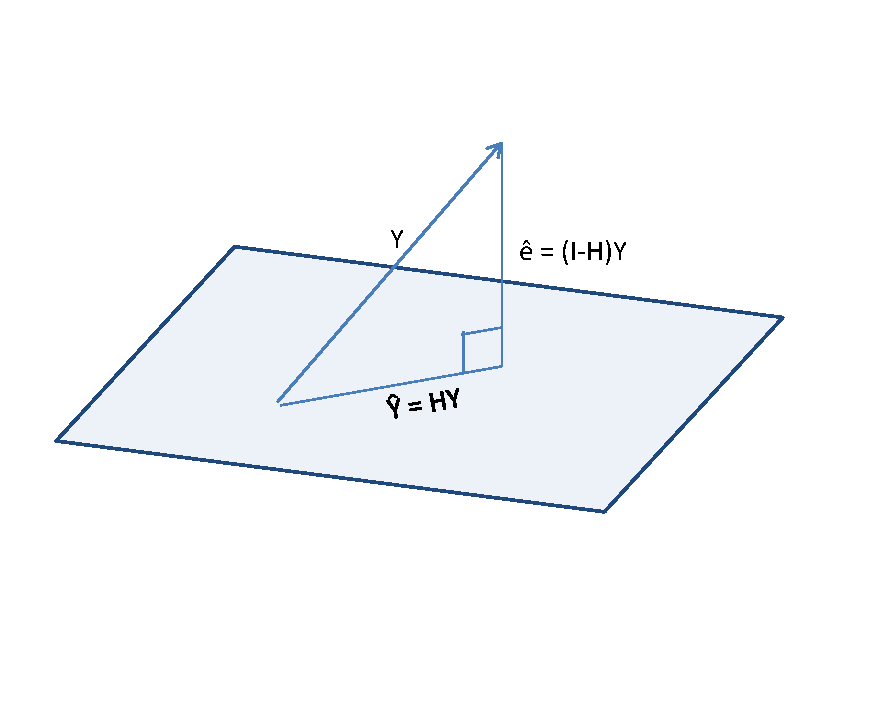
\includegraphics[scale = 0.35]{Chap6-InferenceRLM/Figures/geometrie}
	\caption{Illustration de l'analyse de la variance généralisée}
	\label{fig:geometrie}
\end{figure}



Le théorème de Pythagore donne
$$||\boY||^2=||\boX\hbobeta||^2+||\boY-\boX\hbobeta||^2,$$
o\`u $||\cdot||$ représente la norme (longueur) du vecteur.

Ainsi on retrouve la décomposition:
\begin{eqnarray*}
\boY'\boY&=&(\boX\hbobeta)'\boX\hbobeta+(\boY-\boX\hbobeta)'(\boY-\boX\hbobeta)\\
\Rightarrow\boY'\boY-n\bar{Y}^2&=&\hbobeta'\boX'\boX\hbobeta
+(\boY-\boX\hbobeta)'(\boY-\boX\hbobeta)-n\bar{Y}^2_n\\
&=&\hbobeta'\boX'\boX\hbobeta-n\bar{Y}^2+\hboeps'\hboeps,
\end{eqnarray*}


%\textcolor{red}{Faire une petit exemple ici avant de parler de F, i.e. presenter SCtot et la division en 2 et montrer que c'est plus grand dans un des cas. Ou alors je fais ca en classe...}

On peut utiliser cette décomposition pour obtenir un tableau d'analyse de la variance comme en RLS. Le tableau \ref{table:anova} résume la table ANOVA pour la RLM.


\begin{table}[htb!]
\caption{Tableau d'analyse de la variance dans le cas de la régression linéaire multiple}\label{table:anova}
\centering
\begin{footnotesize}
\renewcommand{\arraystretch}{1.6}
\begin{tabular}{ccccc}\hline
Source & Degrés de liberté & Sommes des carrés & Carrés moyens & $F$ \\ \hline
Modèle & $ddl_1=p$ &
$SC_{reg}=\sum_{i=1}^n(\hat Y_i-\bar Y)^2$ & $CM_{reg}=SC_{reg}/ddl_1$ & $CM_{reg}/CM_{res}$\\
Erreur & $ddl_2=n-p'$ & $SC_{res}=\sum_{i=1}^n(Y_i-\hat Y_i)^2$ & $CM_{res}=SC_{res}/ddl_2$ & \\
résiduelle & & & \\
\hline Totale (corrigée) & $n-1=p+n-p'$ & $SC_{tot}=\sum_{i=1}^n(Y_i-\bar Y)^2$ & &
\end{tabular}
\end{footnotesize}
\end{table}

On peut ensuite tester l'effet global de toutes les variables exogènes, soit
\begin{eqnarray}
H_0:&~&\beta_1=\beta_2=\cdots=\beta_{p}=0\label{H0:Ftest}\\
\mbox{contre\ }H_1:&~&\mbox{au moins un des coefficients n'est pas nul.}\nonumber
\end{eqnarray}

%Sous $H_0$, le mod\`ele de régression ne devrait pas expliquer la variabilité dans les $Y_i$ et donc le ratio $SC_{reg}/SC_{res}$ devrait prendre une petite valeur. Par contre sous $H_1$, le mod\`ele de régression devrait expliquer une partie de la variabilité des $Y_i$ et donc le ratio $SC_{reg}/SC_{res}$ devrait prendre une grande valeur.

Sous $H_0$, la statistique $F$ suit une loi $\mathcal F$ de Fisher-Snedecor avec $p$ degrés de liberté au numérateur et $n-p'$ degrés de liberté au
dénominateur. On rejette donc $H_0$ au niveau $\alpha$ lorsque la statistique
$\mathcal F$ est supérieure ou égale au quantile
$F_{p,n-p';1-\alpha}$.\\


\begin{exemple}
Pour l'exemple \ref{exp_data}, on peut calculer  $SC_{res}=\hboeps'\hboeps=\hat\sigma^2 (n-p')=38,21$, $SC_{tot}=\boY'\boY-n\bar{Y}^2=904,60-20\left(\frac{120,79}{20}\right)^2=175,089$ et $SC_{reg}=SC_{tot}-SC_{res}=136,88.$ On obtient donc le tableau d'analyse de la variance suivant

\begin{table}[htb!]
\caption{Tableau d'analyse de la variance pour l'exemple \ref{exp_data}}
\centering
\begin{footnotesize}
\renewcommand{\arraystretch}{1.6}
\begin{tabular}{ccccc}\hline
Source & Degrés de liberté & Sommes des carrés & Carrés moyens & $F$ \\ \hline
Modèle & $ddl_1=2$ &
$136,88$ & $136,88/2=68,44$ & $68,44/2,247=30,46$\\
Erreur & $ddl_2=17$ & $38,21$ & $38,21/17=2,247$ & \\
résiduelle & & & \\
\hline Totale & $19$ & $175,09$ & &
\end{tabular}
\end{footnotesize}
\end{table}

Pour tester $H_0:\beta_1=\beta_2=0$, on compare $F=30,46$ au quantile $F_{p,n-p'}(1-\alpha)=F_{2,17}(0,95)=3,59$. Comme $30,46>3,59$, on rejette l'hypothèse nulle. On en conclut donc que les meurtrissures de pêche sont liées soit à la hauteur de chute, soit à la masse volumique, soit aux deux.
\end{exemple}


\newpage

\section{Test de réduction du modèle}

Il est plut\^ot rare en pratique que le test $\mathcal F$ de Fisher global ne
rejette pas l'hypoth\`ese $H_0$ donnée par (\ref{H0:Ftest})
que le modèle de régression est
totalement inutile. Cependant, on veut souvent tester si
le modèle peut être réduit. Cela revient à tester
si un sous-modèle plus simple explique une partie suffisamment
grande de la variabilité dans les $Y_i$ pour qu'il ne soit pas
nécessaire d'utiliser le modèle plus complexe. Il s'agit donc de mesurer si
la différence entre les sommes de carrés résiduels des
deux modèles est faible ou élevée.

%Le principe de la somme de carrés résiduels additionnelle permet de tester cette hypoth\`ese de fa\c{}con formelle. L'idée sous-jacente est simple: si les termes qui sont exclus du modèle plus simple expliquent une partie importante de la variabilité dans les$Y_i$, alors la variabilité due à la fluctuation aléatoire ($SC_{res}$) apparaitra beaucoup plus importante dans le mod\`ele simple que dans le modèle complet.

Cette idée se traduit mathématiquement de la manière suivante. Supposons le modèle de régression
multiple standard
$$Y_i=\beta_0+\beta_1x_{i1}+\cdots+\beta_{p}x_{ip}+\varepsilon_i.$$
On désire tester si un modèle comprenant seulement $k<p$ variables exogènes
suffit à expliquer la variabilité dans les $Y_i$. Par souci de simplicité, on suppose que les $k$ variables exog\`enes en question sont $x_1,\ldots,x_k$. Alors on veut tester
\begin{eqnarray}
H_0:~Y_i&=&\beta_0+\beta_1x_{i1}+\cdots+\beta_kx_{ik}+\varepsilon_i\label{H0:ESS}\\
H_1:~Y_i&=&\beta_0+\beta_1x_{i1}+\cdots+\beta_kx_{ik}+\beta_{k+1}x_{i,k+1}+\cdots+\beta_{p}x_{ip}
+\varepsilon_i.\nonumber
\end{eqnarray}
Le mod\`ele donné par $H_0$ est appelé mod\`ele réduit, alors que l'équation présentée
en $H_1$ se nomme mod\`ele complet.

Soit $SC_{res}^{(0)}$ la somme des carrés résiduels obtenue avec
le modèle réduit et $SC_{res}^{(1)}$ la somme des carrés résiduels obtenue avec le
modèle complet. Alors il est toujours vrai que $SC_{res}^{(1)}\le SC_{res}^{(0)}$. Cependant, sous $H_0$,
la différence entre $SC_{res}^{(0)}$ et $SC_{res}^{(1)}$ sera faible, alors que cette même
différence sera élevée sous $H_1$.

Encore une fois, on standardise le rapport
$(SC_{res}^{(0)}-SC_{res}^{(1)})/SC_{res}^{(1)}$ afin d'obtenir une statistique avec une distribution connue sous $H_0$. On obtient
\begin{equation}\label{F:ESS}
F={SC_{res}^{(0)}-SC_{res}^{(1)}\over
\Delta_{dl}\hat\sigma^2_{H_1}},
\end{equation}
où $\Delta_{dl}$ note la différence entre les degrés de liberté de
$SC_{res}^{(0)}$ et les degrés de liberté de $SC_{res}^{(1)}$. Sous l'hypothèse nulle $H_0$ donnée par
(\ref{H0:ESS}), la statistique $F$ en (\ref{F:ESS}) suit une distribution $\mathcal F$ de Fisher avec $\Delta_{dl}$ degrés de
liberté au numérateur et $n-p'$ degrés de liberté au dénominateur. On rejette donc $H_0$ au
niveau de confiance $\alpha$ lorsque $F\ge F_{\Delta_{dl},n-p'}(1-\alpha)$.

%Il est à noter que $n-p'$ réfère au nombre de degrés de liberté de $SC_{res}^{(1)}$, et que $\hat\sigma^2_{(1)}$ réfère au carré moyen résiduel sous $H_1$. Comme il arrive parfois que le \og modèle complet \fg constitue un modèle qui n'inclut pas toutes les $p$ variables exogènes, il faut ajuster la formule (\ref{F:ESS}) en conséquence. C'est pourquoi il est probablement mieux de retenir la forme à droite de la seconde égalité en(\ref{F:ESS}).

On note qu'il existe plusieurs manières de calculer $\Delta_{dl}$:
\begin{enumerate}\item
$\Delta_{dl}=dl(SC_{res}^{(0)})-dl(SC_{res}^{(1)})$;
\item $\Delta_{dl}=$(nbr de paramètres du mod\`ele $H_1$)-
(nbr de paramètres du modèle $H_0$);
\item $\Delta_{dl}=$ nbr de contraintes sur les param\`etres du mod\`ele complet pour
arriver au mod\`ele réduit.
\end{enumerate}
Ainsi, dans le cas présenté en (\ref{H0:ESS}), on aurait
\begin{enumerate}
\item $dl(SC_{res}^{(0)})=n-(k+1)=n-k-1$\\
$dl(SC_{res}^{(1)})=n-p'$\\
Donc, $\Delta_{dl}=n-k-1-n+p'=p'-k-1=p-k$.
\item Param\`etres sous $H_1$: $p'=p+1$\\
Param\`etres sous $H_0$: $k+1$\\
Donc, $\Delta_{dl}=p+1-k-1=p-k$.
\item Les contraintes pour réduire le mod\`ele $H_1$ au mod\`ele $H_0$ sont
$$\beta_{k+1}~=~0,\ldots, \beta_{p}~=~0,$$ c'est-à-dire $p-k$ égalités (contraintes) sur les param\`etres du mod\`ele complet afin d'obtenir le mod\`ele réduit. Donc $\Delta_{dl}=p-k$.
\end{enumerate}

\subsection{Cas particuliers simples}

La très grande majorité des tests d'hypothèses que nous aurons à effectuer dans ce cours
pourrons \^etre exprimés sous la forme $H_0:$ mod\`ele réduit contre $H_1:$ mod\`ele complet. Trois cas particuliers ont des noms spécifiques et méritent d'être étudiés.

\textbf{Test global de la régression}

Le $F$ de la table ANOVA présentée à la dernière section constitue en fait un test de réduction de modèle dans lequel le mod\`ele complet contient toutes les variables exogènes disponibles et le modèle réduit s'écrit simplement comme $Y_i=\beta_0+\varepsilon_i$.  Dans ce cas on peut facilement voir que la statistique $F$ donnée en (\ref{F:ESS}) est égale \`a la statistique $F$ de la table ANOVA. De plus, on déduit aussi facilement que $\Delta_{dl}=p$.

\newpage
\textbf{Tests de $F$ séquentiels}

Il s'agit de tests de réduction de modèles séquentiels pour toutes les variables du jeu de données. On commence avec le modèle nul comme modèle simple et on ajoute séquentiellement chaque variable en testant si elle permet de réduire significativement la somme des carrés résiduelle.

On présente souvent les valeurs de $F$ et valeurs de $p$ associées pour les tests de $F$ séquentiels de toutes les variables d'un jeu de données dans un seul tableau. Les résultats dépendront de l'ordre dans lequel on ajoute les variables.

\begin{remarque}
Dans certains livres et logiciels on parle dans ce cas de sommes de carrés de type I.
\end{remarque}


\textbf{Tests de $F$ ajustés}

On parle de tests de $F$ ajustés quand on teste l'effet de l'ajout de chaque variable, en tenant compte de toutes les autres variables présentes dans le modèle. On dit qu'on ajuste pour toutes les autres variables présentes dans le modèle.

Un test de $F$ ajusté pour la variable $j$ teste donc
\begin{eqnarray*}
H_0:~Y_i&=&\beta_0+\beta_1x_{i1}+\cdots+ \beta_{j-1}x_{i(j-1)} + \beta_{j+1}x_{i(j+1)}+ \beta_kx_{ik}+\varepsilon_i\\
H_1:~Y_i&=&\beta_0+\beta_1x_{i1}+\cdots+ \beta_{j-1}x_{i(j-1)} + \beta_{j}x_{ij}+ \beta_{j+1}x_{i(j+1)}+ \beta_kx_{ik}+\varepsilon_i
\end{eqnarray*}

Ici aussi on présente souvent dans un seul tableau les résultats des tests de $F$ ajustés de toutes les variables d'un jeu de données. Puisqu'on ajuste à chaque fois sur toutes les variables disponibles, les résultats ne dépendront pas de l'ordre dans lequel les variables sont testées.

\begin{remarque}
On parle parfois dans ce cas de sommes de carrés de type II.
\end{remarque}

\begin{remarque}
Dans un test de $F$ ajusté pour la variable $j$, on teste en fait $H_0 : \beta_j=0$ vs $H_1 : \beta_j \ne 0$. On peut d'ailleurs montrer que ce test est équivalent au test $t$ de l'hypothèse $H_0 : \beta_j=0$ basé sur la distribution de $\hat{\bobeta}$ et mentionné à la section \ref{sec:infbetaRLM}.
\end{remarque}

\newpage
\subsection{Point de vue géométrique}

On peut également comprendre les tests de réduction de modèle d'un point de vue géométrique. La statistique $F$ du test est alors construite en standardisant les longueurs des vecteurs appropriés en les divisant par la dimension de l'espace dans lesquels ils vivent (leurs degrés de liberté). La figure \ref{fig:geometrie_gen} montre toutes les quantités impliquées.

\begin{figure}[htb!]
	\centering
		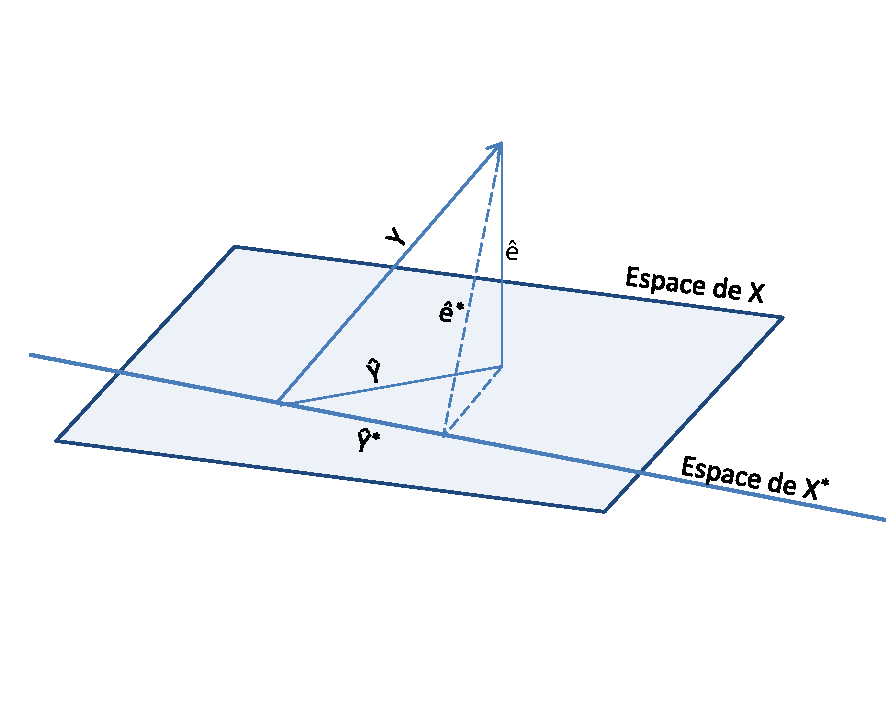
\includegraphics[scale = 0.35]{Chap6-InferenceRLM/Figures/geometrie_gen}
	\caption{Illustration de l'analyse de la variance généralisée}
	\label{fig:geometrie_gen}
\end{figure}

\begin{itemize}
\item[$\bullet$] Le plan Espace de $X$ est l'espace colonne de la matrice d'incidence sous $H_1$.
\item[$\bullet$] La droite Espace de $X^*$ est l'espace colonne de la matrice d'incidence sous $H_0$.
\item[$\bullet$] Le vecteur $\hY$ est $\boX\hbobeta$ sous le modèle complet et se situe dans un espace de dimension $p'$. Ce vecteur constitue la projection orthogonale du vecteur
$\boY$ sur le plan nommé Espace de $X$.
\item[$\bullet$] Le vecteur $\boeps$ est constitué des résidus sous le modèle complet et vit dans un
espace de dimension $n-p'$.
\item[$\bullet$] Le vecteur $\hY^*$ représente le vecteur $\boX\hbobeta$ sous le modèle réduit et évolue dans un espace de dimension $p'-\Delta_{dl}$. Ce vecteur est la projection
orthogonale du vecteur $\boY$ sur la droite Espace de $X$.
\item[$\bullet$] Le vecteur $\boeps^*$ est formé des résidus sous le modèle réduit et
vit dans un espace de dimension $n-p'+\Delta_{dl}$.
\end{itemize}

Le vecteur égal à la différence entre les vecteurs de résidus des
deux mod\`eles est important. Notons $C$ sa longueur. $C^2$ est donc la différence entre les sommes
de carrés résiduels. Ce vecteur vit dans un espace de
dimension $\Delta_{dl}$. La statistique du test $F$ du principe de
somme de carrés résiduels additionnelle est tout simplement
égale \`a $(C^2/\Delta_{dl})/(B^2/(n-p'))$ où $B$ dénote la longueur du vecteur des résidus sous le modèle complet.

\section{Test d'une hypoth\`ese linéaire générale}
\label{sec:hyplingen}

Plusieurs tests en régression linéaire peuvent être exprimés comme une liste de contraintes linéaires sur les valeurs des param\`etres. Soit $\bo{C}$, une matrice de dimension
$r\times p'$, et $\bo{d}$, un vecteur de dimension $r\times1$. Un test d'hypoth\`ese linéaire
générale s'écrit comme
\begin{eqnarray}\label{H0:lingen}
H_0:~\bo{C}\bobeta&=&\bo{d}\\
\mbox{contre\ }H_1:~\bo{C}\bobeta&\neq&\bo{d}.\nonumber
\end{eqnarray}
On peut ré-écrire ce test d'hypoth\`ese sous la forme d'un mod\`ele réduit et d'un mod\`ele
complet de la manière suivante :
\begin{eqnarray*}
H_0:~\boY&=&\bo{Z}\bo{\alpha}+\boeps\\
\mbox{vs\ \ }H_1:~\boY&=&\boX\bobeta+\boeps,
\end{eqnarray*}
où l'équation en $H_0$ est obtenue en (i) résolvant le système d'équations
$\bo{C}\bobeta=\bo{d}$ pour $\bobeta$ et (ii) en substituant la solution trouvée en (i)
dans le modèle $\boY=\boX\bobeta+\boeps$.

%Puisque le test d'une hypothèse linéaire générale est équivalent à tester un modèle réduit contre un mod\`ele complet, on peut utiliser le principe de somme des carrés résiduels additionnelle.
Il est possible de
montrer \citep[voir par e.g.][pp. 44--45 et pp. 60--64]{Sen_Sri:90} que
$$SC_{res}^{(0)}-SC_{res}^{(1)}=(\bo{C}\hbobeta-\bo{d})'[\bo{C}(\boX'\boX)^{-1}\bo{C}']^{-1}(\bo{C}
\hbobeta-\bo{d}).$$
Notez que $\sigma^2[\bo{C}(\boX'\boX)^{-1}\bo{C}']$ est la variance de $\bo{C}\hbobeta-\bo{d}$. Donc
la différence des sommes de carrés résiduels peut \^etre vue comme la longueur du vecteur
qui sépare $\bo{C}\hbobeta$ et $\bo{d}$, standardisée par sa variance. Si la distance entre
$\bo{C}\hbobeta$ et $\bo{d}$ est faible, alors $H_0$ constitue une hypothèse raisonnable, $SC_{res}^{(0)}-
SC_{res}^{(1)}$ prend une petite valeur et on ne rejette donc pas $H_0$. Si $H_0$ n'est pas réaliste, alors
$\bo{C}\hbobeta$ sera éloignée de $\bo{d}$, $SC_{res}^{(0)}-SC_{res}^{(1)}$ prendra une grande valeur
et on rejettera l'hypothèse nulle $H_0$.

On peut maintenant construire la statistique $F$ en utilisant l'équation (\ref{F:ESS}):
\begin{equation*}\label{F:lingen}
F={(\bo{C}\hbobeta-\bo{d})'[\bo{C}(\boX'\boX)^{-1}\bo{C}']^{-1}(\bo{C}\hbobeta-\bo{d})/r\over
SC^{(1)}_{res}/(n-p')}={
(\bo{C}\hbobeta-\bo{d})'[\bo{C}(\boX'\boX)^{-1}\bo{C}']^{-1}(\bo{C}\hbobeta-\bo{d})\over
r\hat\sigma^2_{H_1}},
\end{equation*}
où $r$ note le nombre de lignes de la matrice $\bo{C}$.
Le fait que $\Delta_{dl}=r$ dans ce cas est facile \`a comprendre si on utilise la troisième manière de le calculer, soit le nombre de contraintes sur les param\`etres du mod\`ele complet pour
obtenir le mod\`ele réduit. Sous l'hypothèse $H_0$, $F$ suit une loi de Fisher $\mathcal{F}_{r,n-p'}.$


%\begin{remarque}\label{rem:saslingen}
%Dans l'aide de SAS, on utilise la notation $\bo{L}\beta=\bo{c}$ plut\^ot que
%la notation $\bo{C}\bobeta=\bo{d}$ qui est utilisée par plusieurs livres.
%L'aide de SAS utilise aussi $b$ pour dénoter
%l'estimateur de $\bobeta$ plut\^ot que $\hbobeta$.
%\end{remarque}



